
\nonstopmode

\documentclass{beamer}

\usetheme{metropolis}

%% Sets page size and margins
%\usepackage[a4paper,top=3cm,bottom=2cm,left=3cm,right=3cm,
%		marginparwidth=1.75cm]{geometry}
\usepackage{geometry}
\usepackage{graphicx}
\usepackage{color}
\usepackage{listings}
\usepackage{listings-rust}
\definecolor{comentaryGreen}{rgb}{0,0.6,0}

\definecolor{UniBlue}{RGB}{83,121,170}
\setbeamercolor{title separator}{fg=UniBlue}

%% Language and font encodings %%
\usepackage[utf8]{inputenc}
\usepackage[english]{babel}

\lstset{
         basicstyle=\tiny  ,
         numbers=none,              
         tabsize=1,
         extendedchars=true,         
         breaklines=true,
         keywordstyle=\color{blue},       
         commentstyle=\color{comentaryGreen},
         rulecolor=\color{black},         
         showspaces=false,  
         showtabs=false,   
         showstringspaces=false, 
         xleftmargin=0pt,
         framexleftmargin=0pt,
         framexrightmargin=0pt,
         framexbottommargin=0pt,
 }
%\lstloadlanguages{
%         Rust
%} 

\graphicspath{{res/}}

%gets rid of bottom navigation bars
\setbeamertemplate{footline}[frame number]{}

%gets rid of bottom navigation symbols
\setbeamertemplate{navigation symbols}{}

%\usefonttheme{serif}

\title{Magic of Makefiles}

\date{}
\author{Guy Nankivell}

\begin{document}

	\frame {
		\titlepage
	}

	\frame {

		\frametitle{History of Makefiles}

		\begin{itemize}
			\item Born in 1976 (43 years ago)
			\item Bell Labs Creation
			\item ``Printable, debuggable understandable stuff"
			\item Designed to replace a bevvy of shell scripts
		\end{itemize}

	}

	\begin{frame}

		\frametitle{How it works}
		This is alarmingly simple in its design;
		
		It leverages the syscall \texttt{stat} to check when the output file was
		created. If there are any edits made on files that are \emph{newer} than this,
		it recompiles the files.
		
		This gives the user really granular control over the recompilation phase.

	\end{frame}

	\frame {
		\frametitle{Requirements of a Build System}

		\begin{itemize}
			\item Portable
			\item Efficient (Stop unecessary recompilations)
			\item Language Agnostic (nested projects)
			\item Fast
			\item Modular
			\item Flexible
		\end{itemize}

	}

	\frame{

		\frametitle{Little Note...}

		What I henceforth refer to as `make' is
		the GNU implementation. This is due to being the most common reference
		for \texttt{make} in the wild.
		

	}

	\frame {

		\frametitle{Cornerstone Features of Make}
			\begin{itemize}
				\item Parallel
				\item Text Replacement
				\item Ubiquity
				\item Everyone knows how to use it (Just type \texttt{make}!!)
			\end{itemize}

	}


	\frame {

		\frametitle{Contextualising my Usage}

		\begin{itemize}
			\item C
			\item Fortran
			\item \LaTeX
			\item x86-64 Assembly
			\item Installation Scripts
		\end{itemize}
		Have also used it on...
		\begin{itemize}
			\item Java
			\item F/C\#
			\item Python
		\end{itemize}

}


	\begin{frame}[containsverbatim]

		\frametitle{Anatomy of a Makefile}
		\lstset{basicstyle=\scriptsize\small,language=[gnu] make}
		\begin{lstlisting}
		CONSTANTS =	this that
		JUNK =		*.aux *.snm *.log *.dvi

		target: deps 
			recipe to build

		clean:
			rm $(JUNK)

		.PHONY: clean
		\end{lstlisting}
	\end{frame}

	\frame {

		\frametitle{Okay, but can it work for us?}

		It is used as the build system for the Linux kernel so it must be
		doing something right... How about on modern projects?

		\emph{
		``Those who do not understand Unix are condemned to reinvent it, poorly."
		}
		\begin{itemize}
			\item Good Readability
			\item Easy to implement complex logic
			\item Finding it hard is a symptom of a bad mindset
			\item MASSIVE community using it for js (more than 3 people)
		\end{itemize}

	}

	\frame {
		\frametitle{Node Makefile?}
		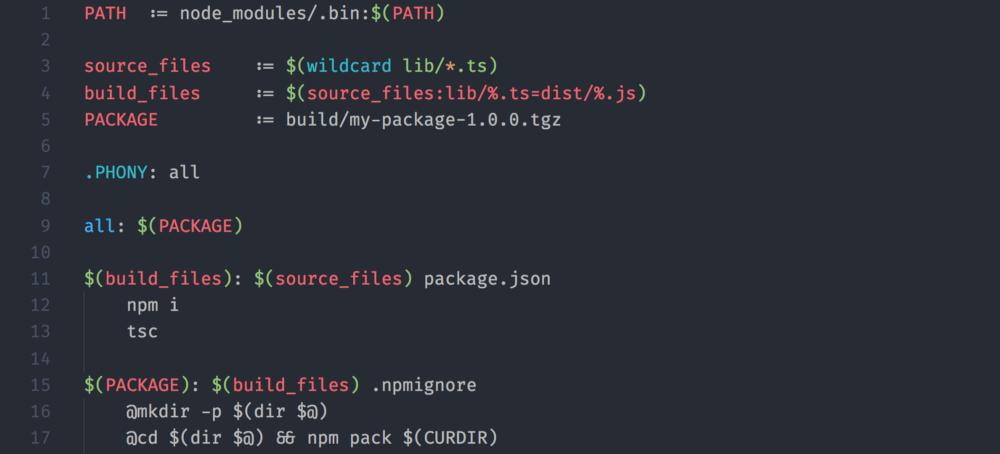
\includegraphics[scale=0.3]{node}

	}

	\frame {

		\frametitle{Drawbacks}
		\begin{itemize}
		\item Arcane Syntax
		\item No Dependency Resolution
		\end{itemize}

	}

	\begin{frame}[containsverbatim]
		\frametitle {Compiling this presentation...}
		\lstset{basicstyle=\scriptsize\ttfamily,language=[gnu] make}
		\begin{lstlisting}
CC =            pdflatex
SRC =           talk.tex
OUT_DIR =       tmp
CFLAGS =        -output-directory $(OUT_DIR)
FILE_REDIR =    /dev/null
FNAME =         out.pdf

all: $(OUT_DIR)
    @ $(CC) $(CFLAGS) $(SRC) > $(FILE_REDIR)
    @ mv $(OUT_DIR)/*.pdf ./$(FNAME)

clean:
    @ $(RM) -r $(OUT_DIR)/

$(OUT_DIR): 
    @ mkdir -p $(OUT_DIR)/

		\end{lstlisting}

	\end{frame}

	\frame {

		\frametitle{Plays nicely with \texttt{vim}}
		From command mode in \texttt{vim} all one has to do to action the
		\texttt{Makefile} in the same directory to which your session is running
		is;
		\begin{center}
			\texttt{:make}
		\end{center}

		Which keeps your editing session alive and allows you to view the
		output of the command and then you need only press enter to drop back into
		editing mode


	}

	\frame {

		\frametitle{\textit{Finis.}}

\begin{center}
			Questions?
\end{center}

	}


\end{document}

